% !TeX root = ..\rapport_13_1.tex
\section{Programdesign}
\subsection{Klassediagram af programdesign}
\begin{figure}[H]
    \centering
    \caption{Klassediagram}\label{fig:ClassDiag}
    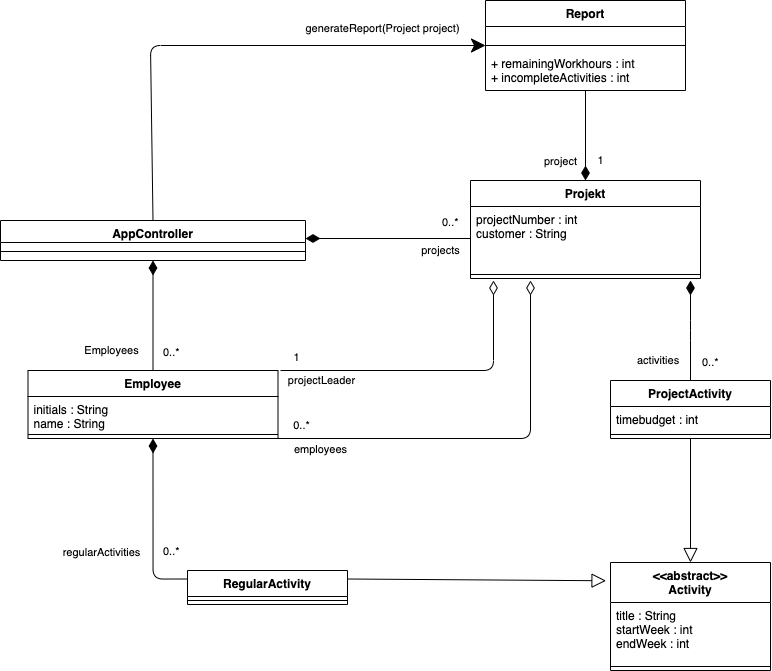
\includegraphics[width = .75\textwidth]{Diagrams/Klassediagram_eng.png}
    % \caption{DANSK udkast af Klassediagram}\label{fig:ClassDiag}
    % 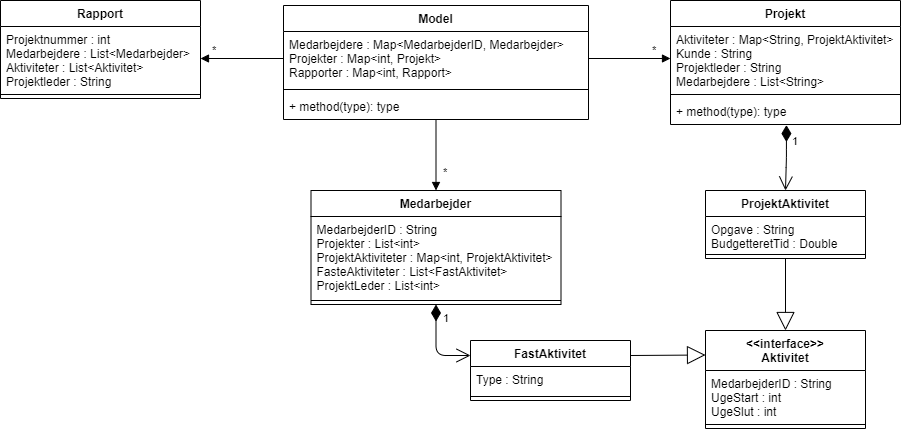
\includegraphics[width = .75\textwidth]{Diagrams/Klassediagram.png}
\end{figure}
\subsection{Sekvensdiagrammer}\label{sec:sequence}
\begin{figure}[H]
    \centering
    \caption{Sekvensdiagram: Opret medarbejder}\label{fig:sequence_register_employee1}
    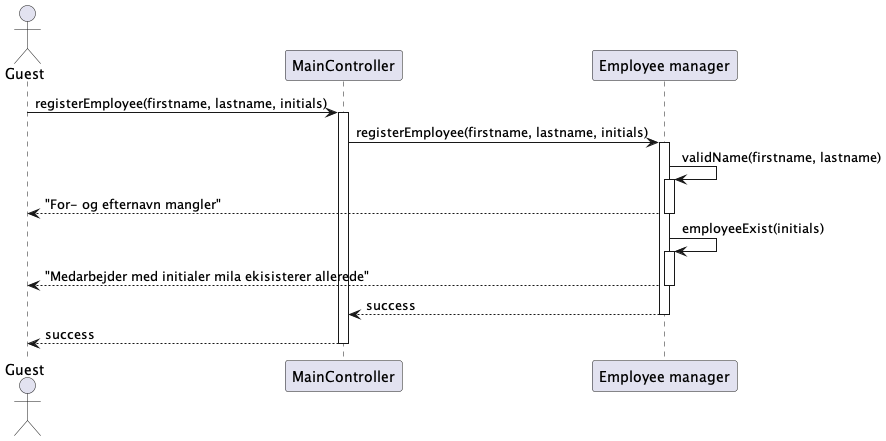
\includegraphics[width = .75\textwidth]{Diagrams/seq_register_employee.png}
\end{figure}
\begin{figure}[H]
    \centering
    \caption{Sekvensdiagram: Opret medarbejder (et andet forslag)}\label{fig:sequence_register_employee2}
    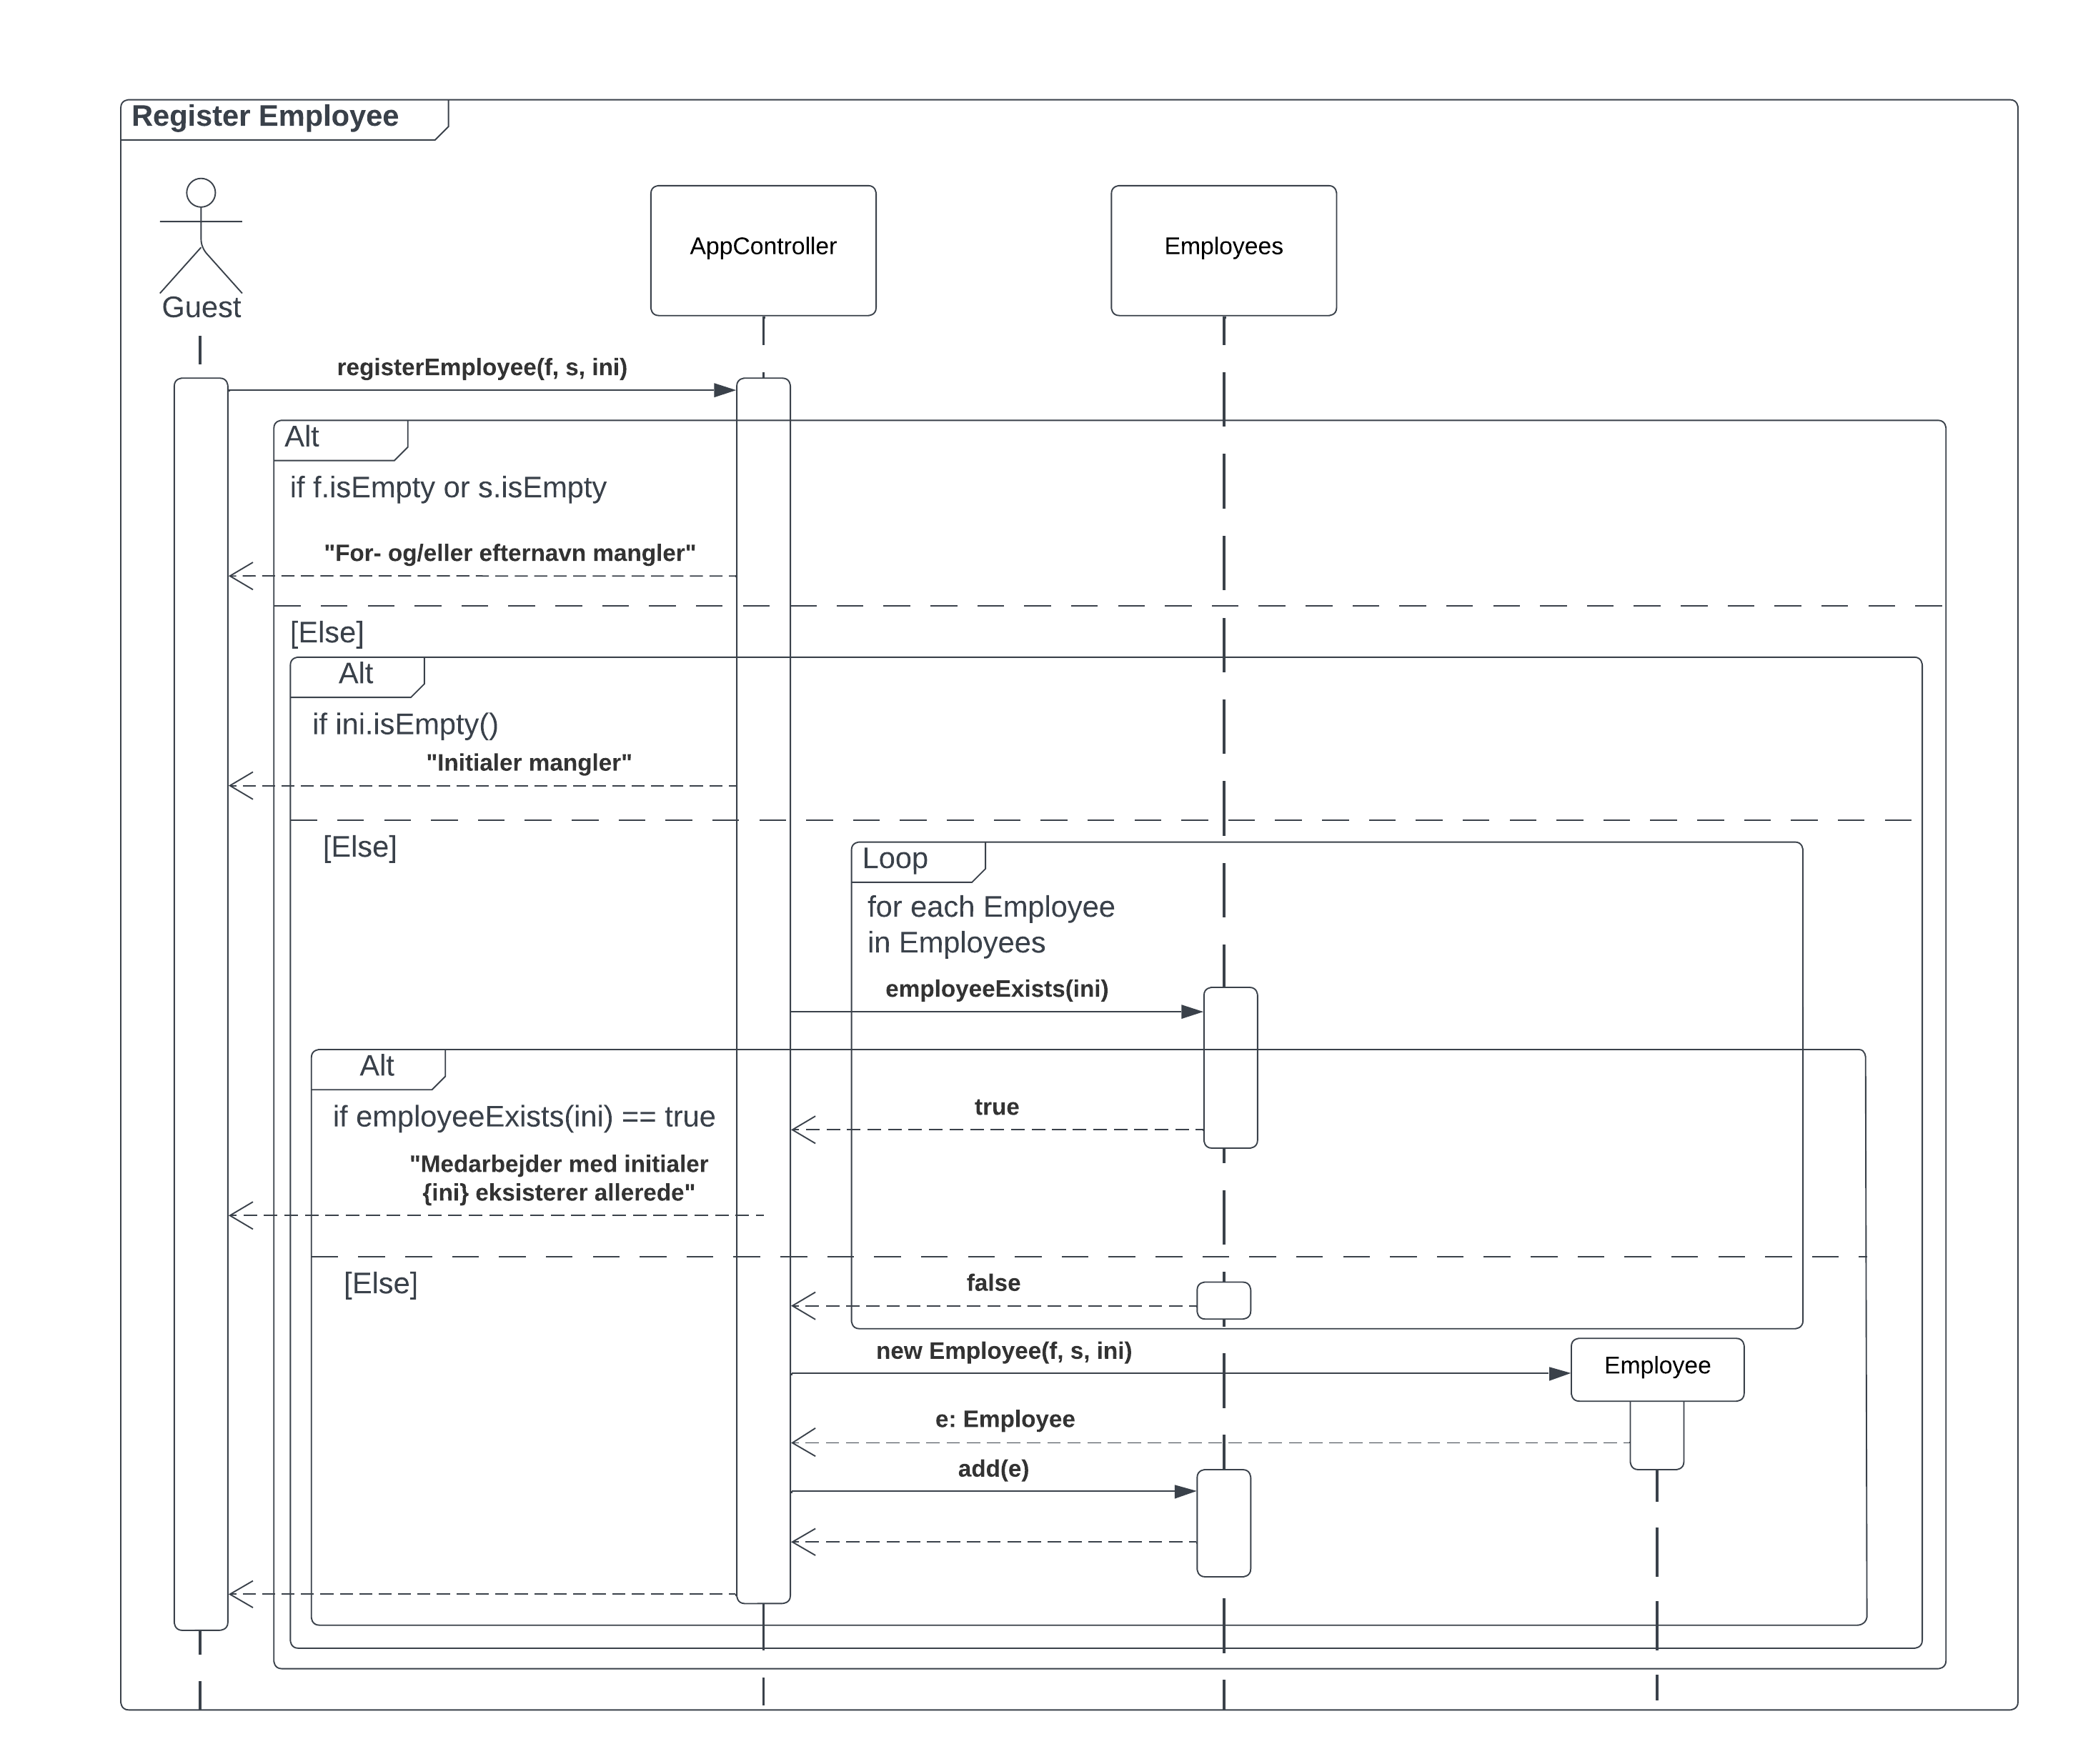
\includegraphics[width = 1\textwidth]{Diagrams/Register Employee.png}
\end{figure}
\begin{figure}[H]
    \centering
    \caption{Sekvensdiagram: Medarbejder login}\label{fig:sequence_login}
    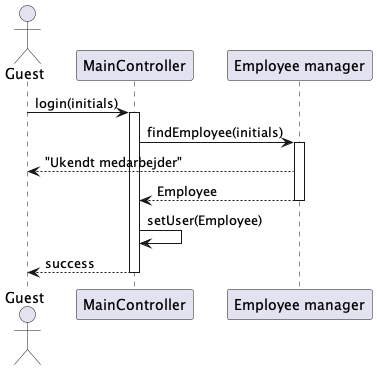
\includegraphics[width = .45\textwidth]{Diagrams/seq_login.png}
\end{figure}
\begin{figure}[H]
    \centering
    \caption{Sekvensdiagram: Medarbejder log ud}\label{fig:sequence_logout}
    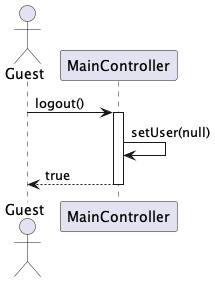
\includegraphics[width = .25\textwidth]{Diagrams/seq_logout.png}
\end{figure}
\begin{figure}[H]
    \centering
    \caption{Sekvensdiagram: Opret projekt}\label{fig:sequence_create_project}
    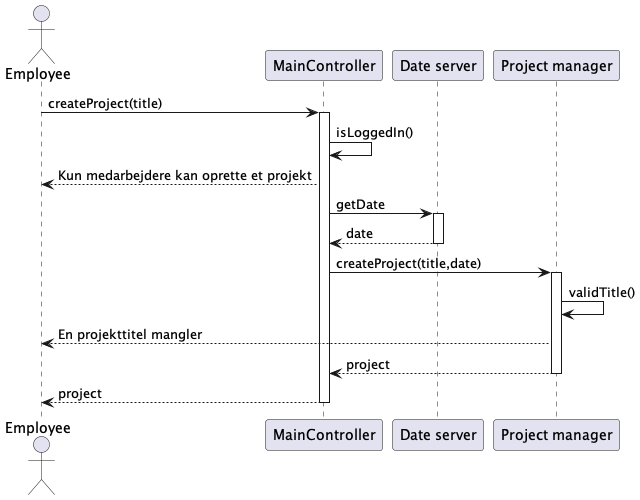
\includegraphics[width = .75\textwidth]{Diagrams/seq_create_project.png}
\end{figure}
\begin{figure}[H]
    \centering
    \caption{Sekvensdiagram: Rediger projekt}\label{fig:sequence_project_edit}
    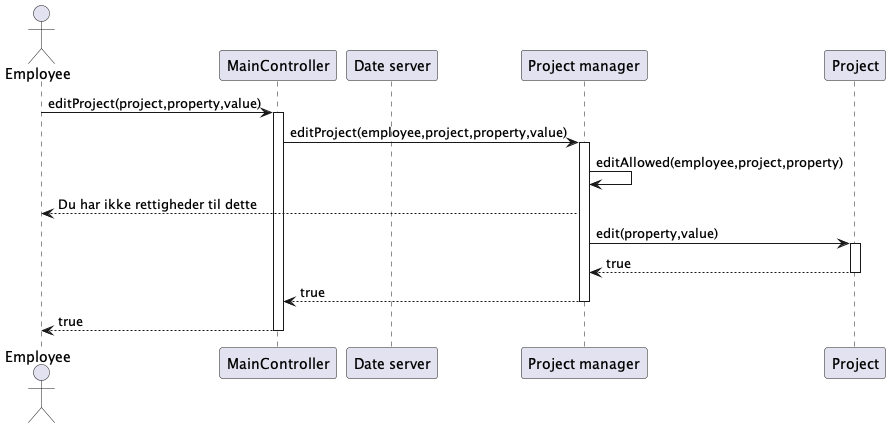
\includegraphics[width = .75\textwidth]{Diagrams/seq_project_edit.png}
\end{figure}
\begin{figure}[H]
    \centering
    \caption{Sekvensdiagram: Medarbejder udpeger sig som projektleder}\label{fig:becomeProjectLeader}
    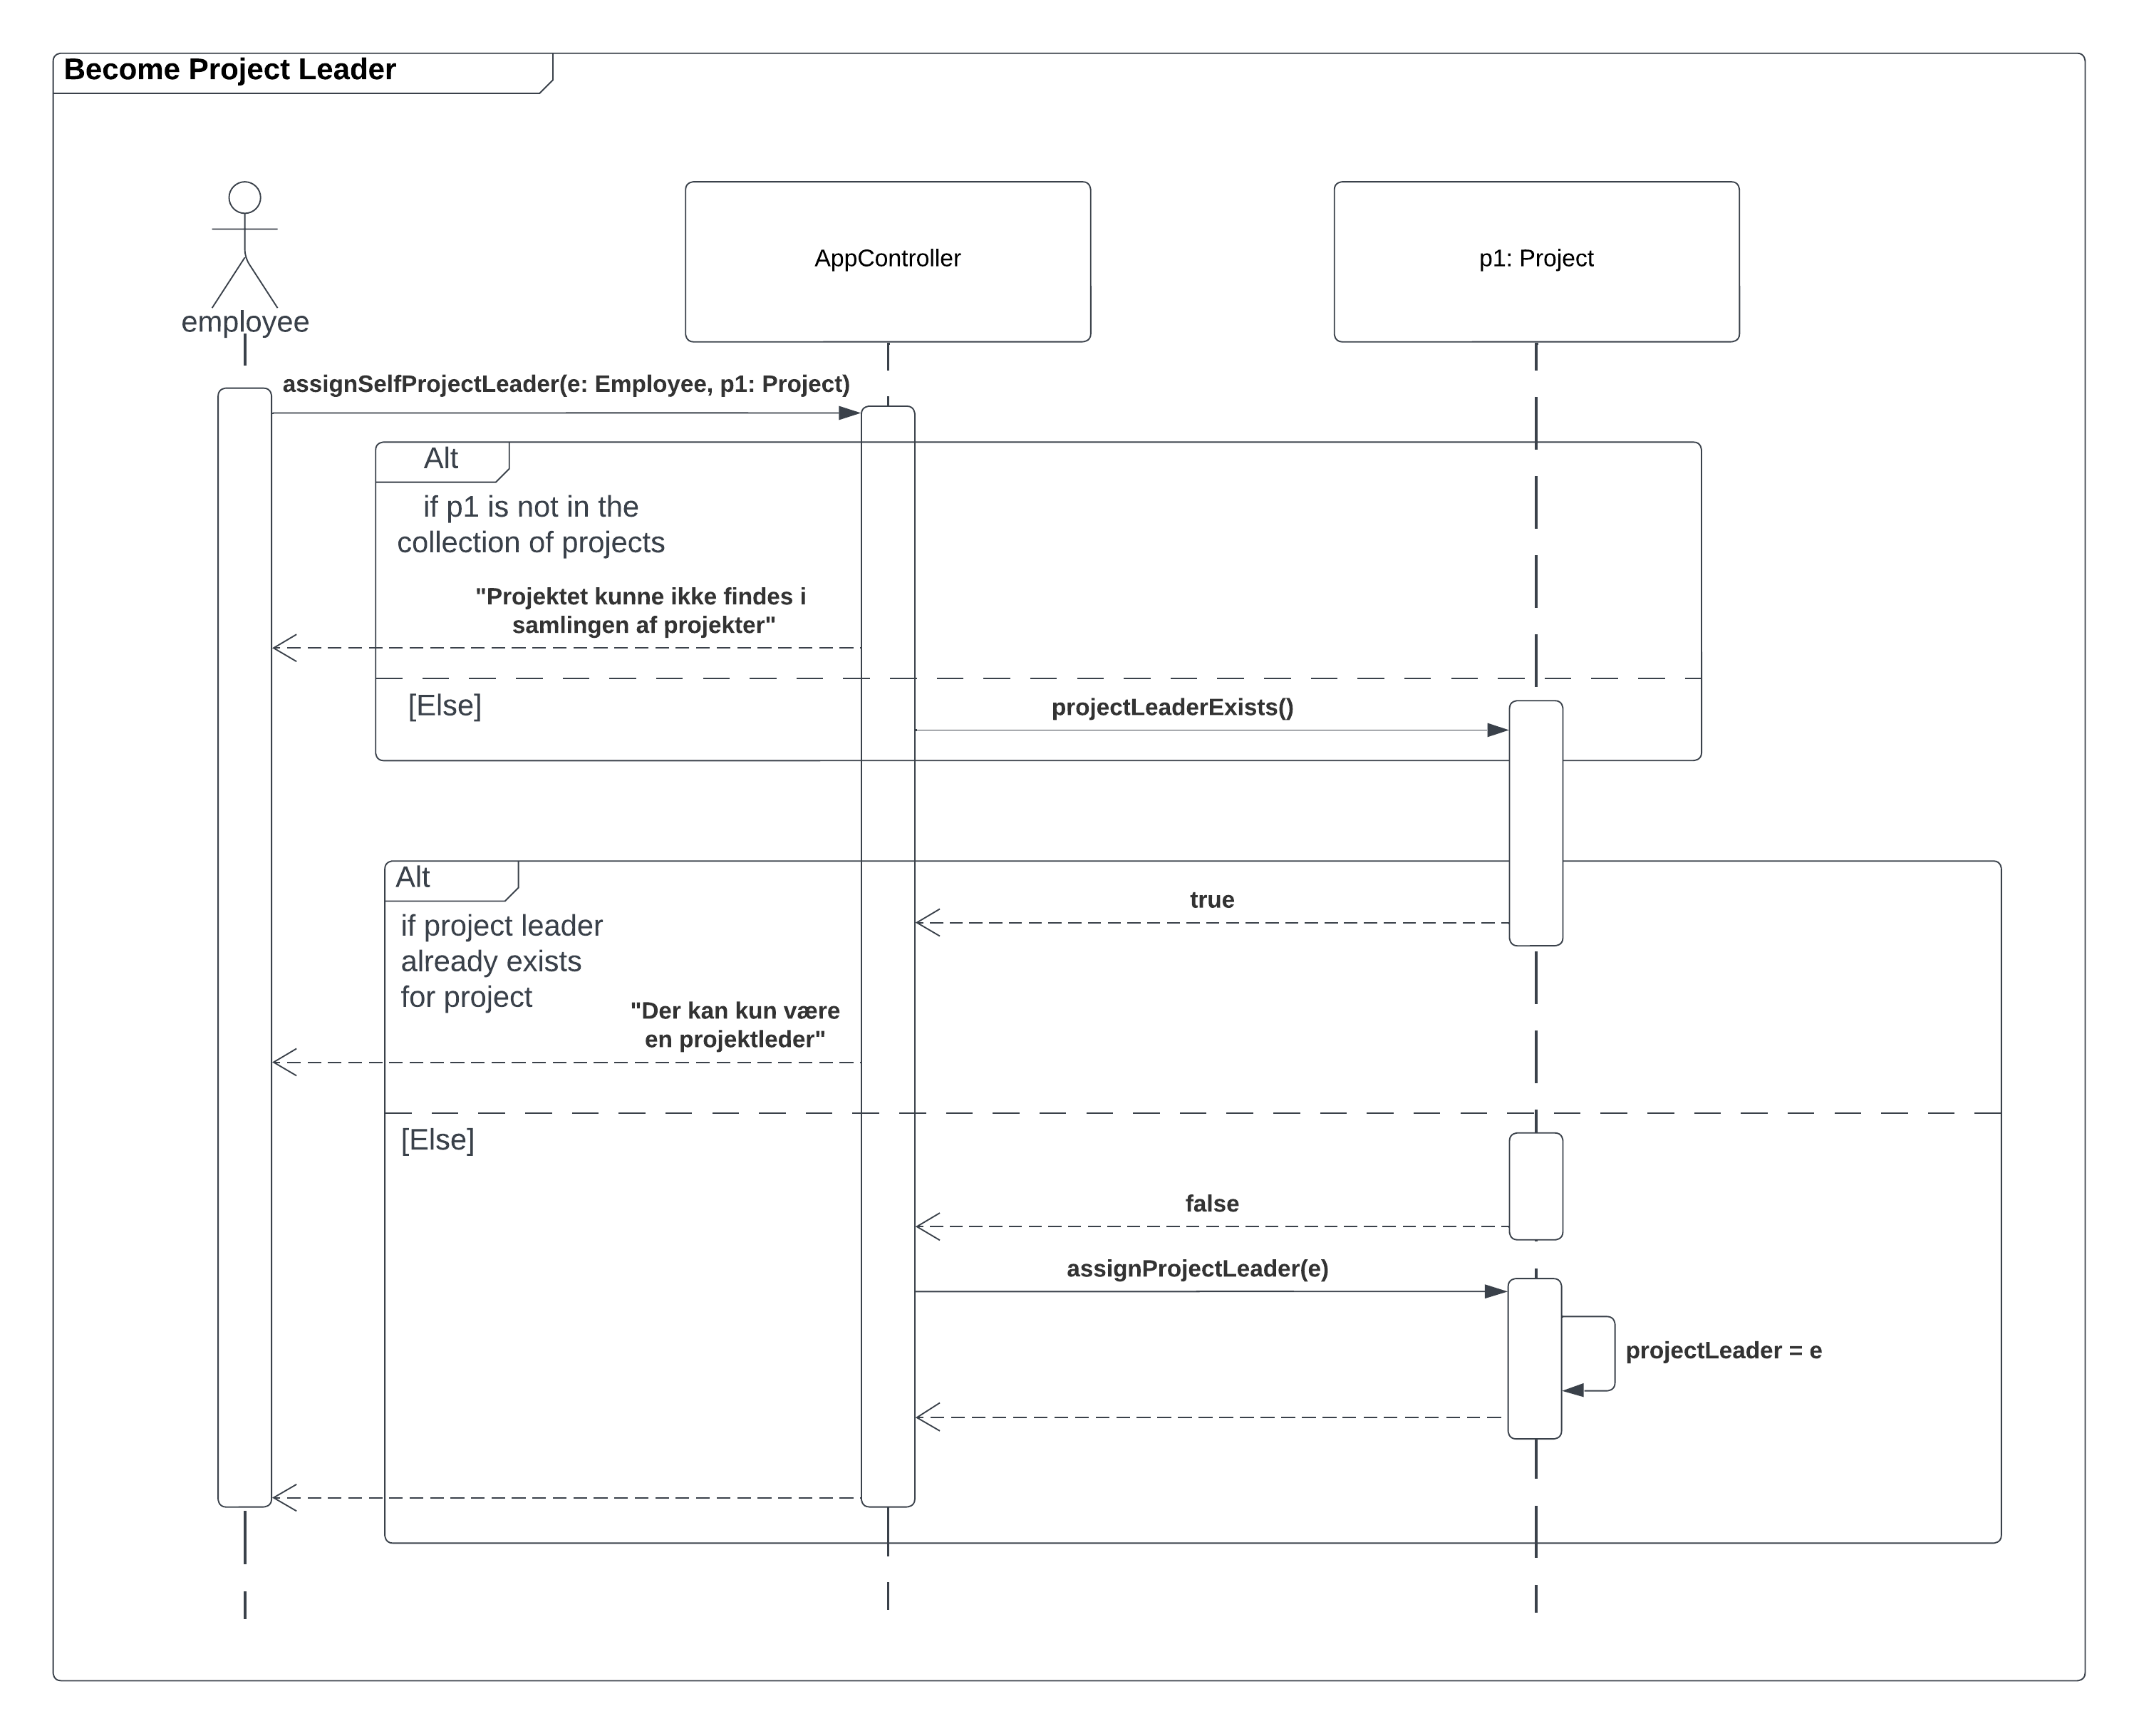
\includegraphics[width = 1\textwidth]{Diagrams/Become Project Leader.png}
\end{figure}